\section{Benchmark Dynamical Systems}
\label{sec:benchmarks}
% 이 섹션에서는 우리 연구에서 다루고자 하는 세 가지 dynamical system model에 대해서 설명할 것이다.
% 우리가 다루는 모델은 전염병 모델 (SIR), 먹이사슬 모델 (Lotka-Volterra)와 같은 잘 알려지고 수식을 다루기 쉬운 autonomous system를 다룬다.
% 위 모델들은 단순하지만, 수학적으로 분석하기에 용이해 우리 방법론의 수리적 해석에 용이하다.
% 우리 방법론의 실용적 유용성에 대해 보이기 위해 우리는 OGTT dynamical system model (Joon Ha, Howard Univ)를 다룬다.
% 이 모델은 OGTT 동안 간, 근육, glucose와 insulin의 dynamics를 

% 각각의 dynamical system들은 시간에 따른 변수들 사이의 상호관계를 모델링한다.
% system의 parameter들은 주로 각 변수들 사이의 상호관계 정도를 나타내게 된다.
% 예를들어, 전염병 모델(SIR)의 경우, parameter는 전염병의 감염률과 회복률을 나타낸다.
% 이 parameter를 아는 것은 현재 질병이 잘 통제되고 있는지, 아니면 더욱 상황이 악화되고 있는지 의사결정을 하는 데에 중요한 지표 역할을 한다.
% 이처럼, system의 parameter를 정확하게 추정하는 것은 다양한 분야에서 중요한 문제다.

% Parameter는 데이터를 관측하는 환경을 정의한다고 할 수 있다.
% 우리는 고정된 환경에서 변수들을 관측할 수는 있지만, 환경 자체를 나타내는 지표를 획득하기는 어렵다.
% 예를들어, 우리는 어느 통제된 환경에서 서식하는 여우와 토끼를 특정 시점마다 셀 수는 있지만, 그 환경에서의 각 종마다의 생장률과 사망률을 나타내는 parameter는 직접 측정할 수 없다. 
% 더욱 실용적으로는, parameter뿐만 아니라, 각 변수들 또한 관측에 어려움이 있다. 
% 한 시점에서의 관측을 위해 많은 비용이 들기 때문에, time-resolution이 매우 커져 sparse 하거나, 어떤 특정 변수는 측정이 불가하거나 비용이 매우 비싸 partial하게만 관측할 수 있는 경우도 존재한다.
% 이러한 관측가능성에서의 문제들은 parameter estimation을 어렵게 만든다.

This section formulates three dynamical systems used to evaluate the proposed parameter estimation framework. 
The Susceptible-Infected-Recovered (SIR) epidemic model and the Lotka-Volterra (LV) predator-prey model serve as foundational autonomous systems that permit rigorous analysis of structural identifiability. 
To demonstrate practical utility, the framework is further applied to the Oral Glucose Tolerance Test (OGTT) model, which captures the complex physiological dynamics of glucose and insulin. 

For each benchmark problem, we explicitly define the state vector $\mathbf{x} \in \mathbb{R}^d$, the unknown parameter vector $\theta \in \mathbb{R}^p$, the governing nonlinear vector field $f(\mathbf{x}, \theta)$, and the partial observation function $h(\mathbf{x}) = x_\mathrm{obs}$ that maps the full state to the observable subspace.

\subsection{SIR Model}
\label{subsec:sir}

The SIR model is a fundamental system of ODEs describing the spread of infectious diseases~\cite{kermack1927contribution}. 
The state vector is $\mathbf{x}(t) = [S(t), I(t), R(t)]^\top$, where $S(t), I(t), R(t)$ represent the susceptible, infected, and recovered populations, respectively. 
The system dynamics are governed by
\begin{equation}
\label{eq:sir}
    \dot{\mathbf{x}}(t) = f(\mathbf{x}(t), \theta) = 
    \begin{bmatrix}
        -\beta \frac{I(t)S(t)}{\bar{N}(t)} \\[6pt]
        \beta \frac{I(t)S(t)}{\bar{N}(t)} - \gamma I(t) \\[6pt]
        \gamma I(t)
    \end{bmatrix},
    \quad t \in [0, T],
\end{equation}
where the parameter vector $\theta = [\beta, \gamma]^\top \in \mathbb{R}^2$ consists of the infection rate $\beta > 0$ and the recovery rate $\gamma > 0$. 

We assume that the total population $\bar{N}(t)$ is conserved over time. 
This implies that for any initial condition $S_0, I_0, R_0 \ge 0$, the sum remains constant:
\begin{equation}
\label{eq:sir_conserve}
    \bar{N}(t) = S(t) + I(t) + R(t) = S_0 + I_0 + R_0 \equiv \bar{N}.
\end{equation}
In our experiments, $\bar{N}$ is assumed to be a known constant ($\bar{N}=50$).
This linear constraint strictly bounds the feasible region of the hidden state, as $I(t) \leq \bar{N}-S(t)$.
This restriction significantly reduces the effective search space for hidden state estimation.

The basic reproduction number, $\mathcal{R}_0 := \beta / \gamma$, governs the qualitative behavior of the system. 
The value $\mathcal{R}_0 = 1$ serves as a bifurcation threshold: if $\mathcal{R}_0 > 1$, the infected population $I(t)$ forms a peak ($\dot{I} > 0$ initially), whereas if $\mathcal{R}_0 \le 1$, $I(t)$ decreases monotonically. 
To ensure the parameter estimation framework is evaluated without bias toward a specific dynamical regime, the simulation datasets are explicitly constructed to span both sides of this threshold (detailed sampling distributions for $\beta$ and $\gamma$ are deferred to Section \ref{sec:experiments}).

Under the partial and sparse observation setting, %(Section~\ref{subsec:obsmodel}), 
we assume that only the susceptible population $S(t)$ is observable. 
The observation function is defined as a projection $h(\mathbf{x}(t)) = x_\mathrm{obs}(t) = S(t)$.
In practice, this continuous state is sampled on a sparse grid (e.g., $\Delta t=20$).

Due to the population conservation constraint in Equation~\ref{eq:sir_conserve}, the recovered population $R(t)$ is completely determined by $S(t)$ and $I(t)$. 
Consequently, the hidden state reduces to the infected population, $x_{\mathrm{hid}}(t) = I(t)$.

Figure~\ref{fig:sir_traj} illustrates trajectories of the SIR model alongside the partial and sparse observations, highlighting how the system's behavior shifts depending on $\mathcal{R}_0$.
As shown in the figure, while the trajectories of $S(t)$ decrease monotonically in both scenarios, their geometric shape differ.
When $\mathcal{R}_0>1$, the hidden state $I(t)$ undergoes a bell-shaped epidemic peak, which induces a steep, sigmoidal drop in $S(t)$.
Conversely, when $\mathcal{R}_0 < 1$, $I(t)$ decays monotonically, resulting in a much flatter, gradual decrease in $S(t)$.
This shape difference implies that even under the partial and sparse observation setting, the data points retain sufficient structural footprint to identify the governing parameters $\theta$.


\begin{figure}[H]
  \centering
  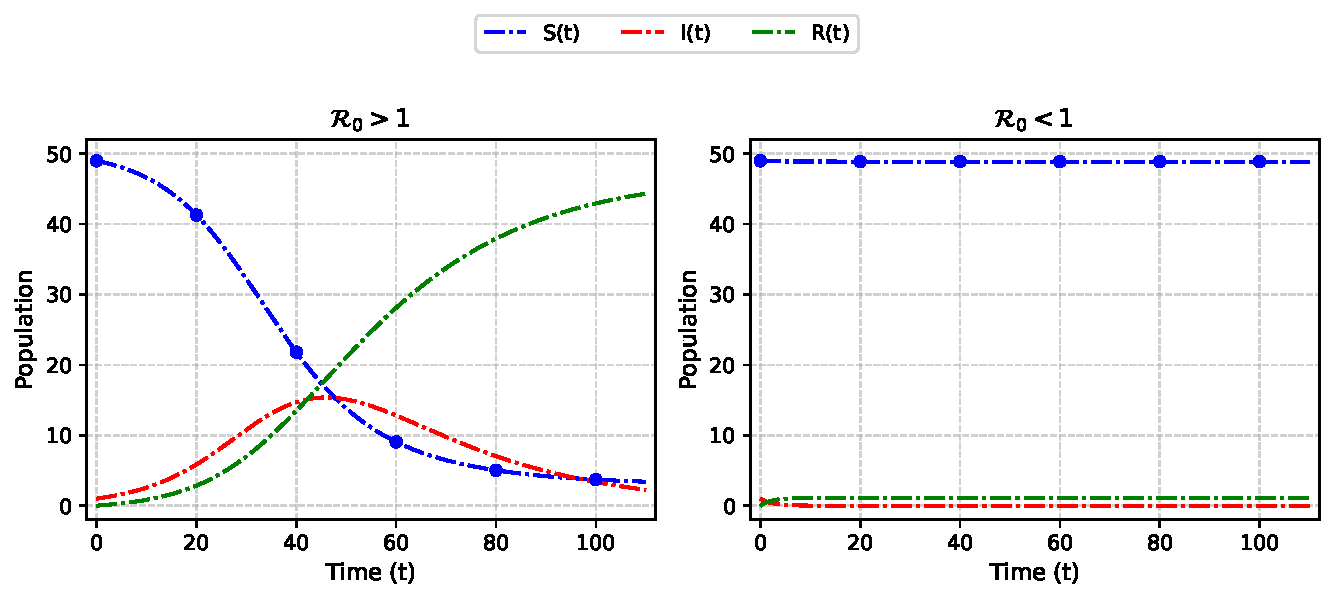
\includegraphics[width=\textwidth]{figures/sir_trajectories.pdf}
  \caption{Trajectories of the SIR model with $\mathcal{R}_0>1$ (Left) and $\mathcal{R}_0 < 1$ (Right). 
  Dash-dot lines denote the continuous simulation of susceptible ($S(t)$), infected ($I(t)$), and recovered ($R(t)$) populations.
  To strictly minimize approximation errors, the simulation is generated via a high-order numerical solver, specifically the explicit Runge-Kutta method of order 5(4)~\cite{dormand1980family}.
  Dots represent the partial and sparse observations sampled over the time interval $[0, 110]$ with a sparse time step of $\Delta t = 20$, which constitute the data available to our framework for parameter inference.
  The contrasting dynamics illustrate the bifurcation governed by $\mathcal{R}_0$:
  an epidemic outbreak regime on the left ($\beta=0.15, \gamma=0.05 \implies \mathcal{R}_0 =3.0$), characterized by a bell-shaped peak of $I(t)$ that induces a steep, sigmoidal drop in $S(t)$, versus a decay regime on the right ($\beta=0.05, \gamma=0.35 \implies \mathcal{R}_0 \approx 0.14$), where $I(t)$ decays monotonically, leaving $S(t)$ relatively flat and gradually decreasing.}
  \label{fig:sir_traj}
\end{figure}
% 흑백 프린트 하니까 구분이 잘 안 됨. 컬러맵 수정 필요

\subsection{Lotka-Volterra Model}
\label{subsec:lotka-volterra}

The Lotka-Volterra (LV) model is a periodic dynamical system describing the interaction between prey and predator populations~\cite{lotka1925elements, volterra1927fluctuations}. 
The state vector is $\mathbf{x}(t) = [x(t), y(t)]^\top$, where $x(t)$ and $y(t)$ represent the prey and predator populations, respectively. 
The system dynamics are governed by
\begin{equation}
\label{eq:lv}
    \dot{\mathbf{x}}(t) = f(\mathbf{x}(t), \theta) = 
    \begin{bmatrix}
        \alpha x(t) - \beta x(t)y(t) \\[6pt]
        \delta x(t)y(t) - \gamma y(t)
    \end{bmatrix},
    \quad t \in [0, T],
\end{equation}
where $x(t)>0$, $y(t)>0$ and the parameter vector is $\theta = [\alpha, \beta, \delta, \gamma]^\top \in \mathbb{R}^4_{>0}$. 
These parameters represent the prey birth rate $\alpha$, the predation rate $\beta$, the predator reproduction rate $\delta$, and the predator death rate $\gamma$.

The LV model provides a critical comparison to the SIR model not only in its oscillatory dynamics but also in its structural constraints. 
While the SIR model benefits from the linear population conservation ($I(t) \le \bar{N} - S(t)$) that strictly bounds the feasible region of the hidden state, the LV system lacks such trivial linear bounds. 
Instead, its trajectories are strictly confined to a level set of a nonlinear invariant manifold defined by the energy function:
\begin{equation}
\label{eq:lv_conserve}
    V(x,y) = \delta x - \gamma \ln x + \beta y - \alpha \ln y.
\end{equation}
Along any valid trajectory, this quantity remains constant $C>0$ such that $V(x(0), y(0)) \equiv C$.
Critically, this nonlinear constraint is explicitly coupled with the parameters $\theta$.
This implies that even if the prey $x(t)$ is observed, the feasible region for the hidden state $y(t)$ cannot be narrowed down without simultaneously identifying $\theta$. 
Consequently, parameter estimation and hidden state inference for the LV model formulate a fundamentally more ill-posed problem than for the SIR model.

Under the partial and sparse observation setting, we assume that only the prey population $x(t)$ is observable, that is, the observation function is defined as a projection $h(\mathbf{x}(t)) = x_\mathrm{obs}(t) = x(t)$.
A highly sparse observation regime is employed to evaluate the parameter estimation framework. 
Specifically, the observed data is restricted to a fixed time interval $t \in [0, 20]$ on a discrete grid of $N=10$ evenly spaced points, resulting in a coarse time step of $\Delta t \approx 2.22$.
To construct simulation datasets that capture the system's periodic nature without altering this fixed grid, we control the initial conditions based on the relative energy level $\Delta V = V(x(0), y(0)) - V(x^*, y^*)$, where $(x^*, y^*) = (\gamma/\delta, \alpha/\beta)$ is the equilibrium point. 
In practice, these initial conditions are generated via a rejection sampling scheme. 
Candidate coordinates $(x_0, y_0)$ are drawn uniformly from a bounded box surrounding the equilibrium point, and a candidate is accepted only if its relative energy strictly satisfies $C_{\min} \le \Delta V \le C_{\max}$. 
Here, the lower bound $C_{\min} > 0$ explicitly excludes trivial, near-linear harmonic oscillations, ensuring the dataset maintains a baseline level of nonlinearity. 
Conversely, the upper bound $C_{\max}$ mathematically guarantees that at least one full closed orbit is encompassed within $T=20$. 
Detailed specifications regarding the parameter distributions and exact boundary values for dataset generation are deferred to Section \ref{sec:experiments}.

This energy-based sampling strategy explicitly governs the difficulty of the inverse problem.
For small perturbations near the equilibrium, the system exhibits near-linear harmonic oscillations with a fundamental frequency $\omega_0 = \sqrt{\alpha\gamma}$. 
Under our parameter configuration, the corresponding minimum period is $T_0 \approx 7.85$, meaning the discrete grid ($\Delta t \approx 2.22$) places roughly 3.5 observation points per cycle. 
This sampling rate safely satisfies the \emph{Nyquist-Shannon sampling theorem}~\cite{shannon2006communication}, ensuring that the continuous dynamics can be adequately resolved.

However, as $\Delta V$ increases, the nonlinearities dominate, and the orbits degenerate into relaxation oscillations. 
In the time domain, these high-energy trajectories exhibit pronounced stiffness, characterized by extremely sharp, rapid transient spikes followed by slow recoveries. 
According to the Nyquist-Shannon sampling theorem, capturing such rapid transitions necessitates a substantially higher Nyquist frequency. 
Consequently, the fixed discrete grid falls critically short of this requirement, inducing severe temporal aliasing. 
This undersampling effectively obliterates the local gradient information during the peaks, meaning the true system dynamics cannot be recovered from local temporal differences alone. 
Thus, our framework is explicitly challenged to leverage the global nonlinear physical constraint \eqref{eq:lv_conserve} as an inductive bias, demonstrating its capacity to reconstruct the hidden state and parameters from the underlying topological geometry rather than highly aliased local transitions.

Figure \ref{fig:lv_traj} illustrates the core challenge of the LV model under this high-energy state.
While the continuous full state $\mathbf{x}(t)$ traces a closed orbit along the nonlinear manifold (Figure~\ref{fig:lv_traj}, Right), only the highly sparse and aliased observations $\left\{x_\mathrm{obs}(t_i)\right\}_{i=0}^{9}$ are available for inference (Figure~\ref{fig:lv_traj}, Left).
Notice how the fixed sampling grid severely misses the sharp nonlinear peaks, demonstrating the temporal aliasing phenomenon.
Thus, the underlying task demands the implicit reconstruction of this global nonlinear geometry solely from these sparse, localized observations.


\begin{figure}[t]
  \centering
  
  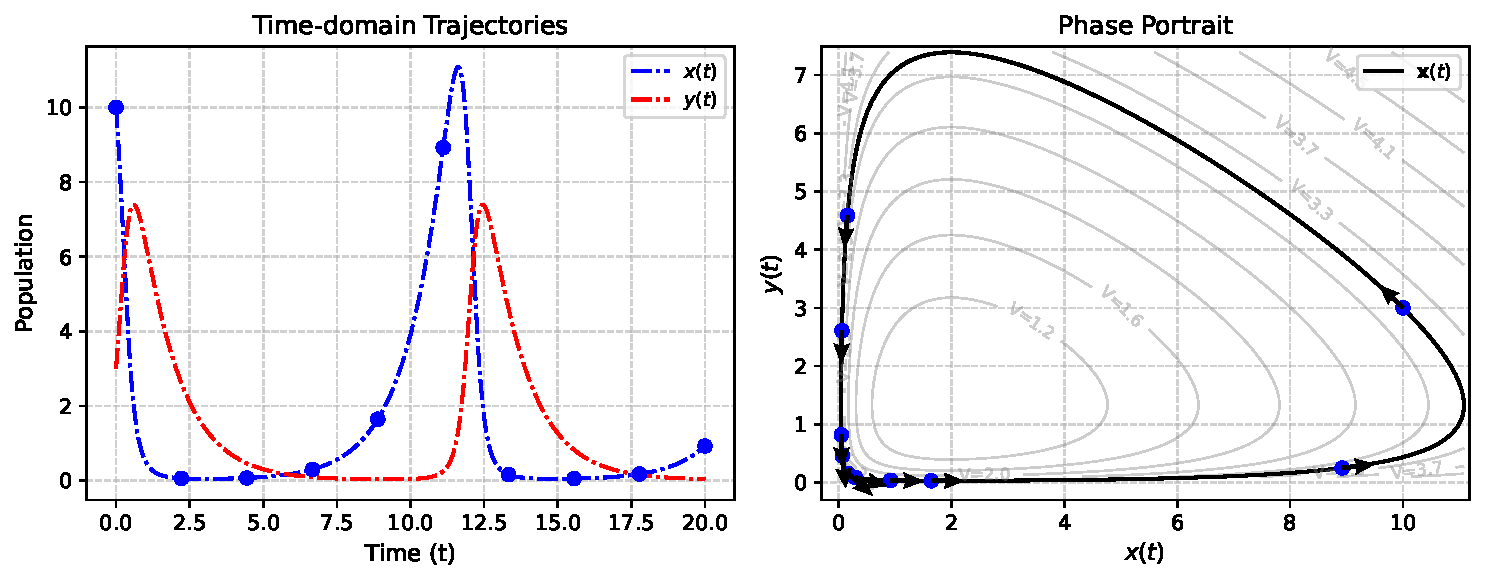
\includegraphics[width=\textwidth]{figures/lv_trajectories.pdf}
  \caption{Trajectories and phase portrait of the Lotka-Volterra model.  
    (Left) Time-domain trajectories of the observed prey $x(t)$ and hidden predator $y(t)$. 
    Dots indicate the sparse observations of $x(t)$, sampled at $N=10$ equally spaced points over the time interval $t \in [0, 20]$. 
(Right) Phase portrait in the $x-y$ plane. 
The continuous state evolution $\mathbf{x}(t)$ forms a closed orbit along the level set of the energy function $V(x,y)$ (background contours). 
The continuous trajectories were generated via the explicit Runge-Kutta method of order 5(4)~\cite{dormand1980family} with parameters $\alpha=0.8, \beta=0.6, \delta=0.4, \gamma=0.8$ and initial conditions $x(0)=10.0, y(0)=3.0$. 
This configuration yields a high energy level of $V(x(0), y(0)) \approx 3.08$, visually demonstrating how the discrete sampling grid fails to capture the sharp transient spikes.}
  \label{fig:lv_traj}
\end{figure}


\subsection{OGTT model}
\label{subsec:ogtt}

To be written....